\chapter{UX Design Cycle 3}
\label{ch:ux3-cycle_report}

The User Experience Design Cycle 3 plan and results discussed here. \\

\section{Research Questions}

This section shows the list of sub research questions considered for each main research question. In the case of the first primary research question, i.e., with displaying results for a single project from multiple static analysis tools, the following are the sub research questions. \\

\begin{enumerate}
\item Do users prefer bug icons or list view for bugs in same file?
\item Do users prefer to see bugs one by one or at once in the context of multiple bugs at the same time?
\item Does vertical view help in getting an overview of the presence of multiple bugs over horizontal views?
\item Do users prefer for table view over text description shown for multiple bugs at a line of code?
\item In context of same bug identified but with different line numbers, would have ‘similar bugs’ in bug description with on click pops up similar bug description boxes at the identified line or a list at the bottom help user in locating actual line where bug exist?
\end{enumerate}

Next, in the case of the second main research question, i.e., with feedback while bug fixing is on-going, the following are the sub research questions. \\

\begin{enumerate}
\item How usable are each feedback functionality compared to the scenario of using unified UI to native UIs?
\item Does alert notification help in fixing more bugs in contrast to its absence in current tools UI?
\item Does MSAT UI with five different feedback mechanisms helps in fixing the bugs in a faster way in comparison to using multiple tools with native user interfaces?
\item Does MSAT UI with five different feedback mechanisms helps in fixing more bugs in comparison to using multiple tools with native user interfaces?
\end{enumerate}

Finally, in the case of the third main research question, i.e., with carrying traceability of bug fixing, the following are the sub research questions. \\

\begin{enumerate}
\item Do users prefer having multiple windows to single window in tracing previous bug fixes in a method?
\item Do users be able to keep up in state of workflow as tools scale?
\item While tracing previous bug fixes in a method, do users prefer a table view to a before/after windows?
\end{enumerate}

Also,
\begin{enumerate}
\item Do users prefer having tool names in general?
\end{enumerate}

\section{User Study Process and Results}

This section explains the user scenario and questionnaire used during the user study.

\subsection{Metrics Analysed}

\subsubsection{Quantitative measurements}  

\begin{enumerate}
	\item Task Success: Whether the user able to complete the respective task or not?
	\item For each research question, ask users to evaluate the solution idea in terms of perceived usability on a Uni-polar Likert scale of 0-10. Scale: 0 – worst, 10 – best, in comparison to alternative solution idea provided.
\end{enumerate} 

\subsubsection{Qualitative measurements} 

Usability: Ask the user to provide feedback through cognitive walkthrough process about problems faced while using the prototype and get insights about the solution idea. \\

\subsection{User Study}

\subsubsection{Pre-test}

By first, the user background is verified with the pre-test questionnaire whether he/she is the right candidate to consider for user study. The ideal choice is the user who has computer science studies background and programs software projects. Also, we examine whether the user has used any static analysis tools and if so, the relationship between their favourite tool and usability is found out. \\

Questionnaire: \\

\begin{enumerate}
\item How often does the user do software development (i.e., coding)?
\item Have the user used static analysis tools?
\item What tools have the user used?
\item Is it IDE integrated tool or any other dedicated tools such as FindBugs, PMD.
\item Do the user ever try to use different tool based?  If no, why?
\item If yes, why? Also, what challenges did they face while using tools separately?
\item Which is the user’s favourite one? 
\item Why is it favourite? Any correlation to its better user interface feature?
\end{enumerate}

\textbf{Results}: \\

There are five users participated in this user study phase. Everyone has Computer Science background with a bachelor’s degree, and also, two users have sound professional experience. All five users are pursuing master’s degree in computer science at the time of this user study. \\

Out of five, three users almost code daily, and two users code three days and two days in a week. Two users have used static analysis tools, and others do manual testing by writing test cases programmatically for their codebase. However, the ones who have not used static analysis tools so far are still aware of its concept during their studies.  The ones who have used static analysis tools are IDE integrated and CLI tool. Although none of them have used multiple static analysis tools for a single project so far, expressed the importance of it. This lead to the discussion of the primary research questions, it surprised us by knowing the users are excited about the thesis topic, once revealed or help them understand the topic. As users have not explored much tools, they have no favourite one unless the one they are using but expressed the importance of usability as in better understandability of bug findings and should ease them in bug fixing workflow in general. \\

Now, we ask the user to assume they are working on a project and want to find bugs in their code. There are ten tools linked to their codebase to have better coverage of vulnerabilities. Next, walk through three main research questions concerning its user interface one by one with their sub research questions and evaluate their solution ideas. \\

Prototypes are made based on solution ideas, i.e., wireframes using Balsamiq software tool. They are presented to user one after other in random order. Then a cognitive walkthrough is carried out with think-aloud process during user study. \\

Now let us walk through each research question. 

\subsubsection{RQ 1: How to display the results of the same codebase from different analysis tools?}

As part of this research question, there are five sub research questions considered. Among the five, the first four sub research questions and their solution ideas are evaluated with similar pattern of User Scenario, Task, Success Criteria and Follow up as mentioned below. \\

\clearpage
\textbf{User Scenario}: \\

The following user scenario is presented to the user, assume as a software developer working on a project called “Alpha”. On the next working day, the user is about to see analysis results from multiple tools, and their primary intention is to make their codebase bug free. \\

\textbf{Task}: \\

After mentioning the user scenario, a task, i.e., “What are the bugs reported for file XSSFilter.java?” is given for the user to perform on the provided prototype which represents a solution idea. \\

\textbf{Success Criteria}: \\

Success Criteria determines whether the user performs the given task, which provides the desired outcome. In this case, the user reports the names of bugs, i.e., XSS\_Config, JSP reflected vulnerability and HttpSession. \\

\textbf{Follow up}: \\

Further, once the user declares he has completed the task on all provided solution ideas for a research question. A set of follow up questions are asked to evaluate the solution ideas. \\

\begin{enumerate}
\item Among the solution ideas presented, which one does the user feel convenient (easy to use) with for the given task?
\item Why is it the mentioned solution idea is convenient?
\item How do the user rate in terms of perceived usability ranging from O, be lower to 10 be high for provided solution designs in comparison? \\
\end{enumerate}

\noindent \textbf{RQ 1-1: Do users prefer bug icons or list view for bugs in same file?} \\

\textbf{Solution Ideas - [ bug icon, list ]}: \\

We evaluate the designs representing the solution ideas, i.e., bug icon and list against each other with the user study process pattern, i.e., User Scenario, Task, Success Criteria and Follow up, as mentioned earlier. \\

The ‘bug icon’ idea is about having a bug icon in the gutter, and user clicks to see the bug description at a particular line. This idea could be well understood, looking at following \autoref{fig:S31_next1} or a complete prototype images added in appendix. \\


\begin{figure}[hbt!]
	\centering
	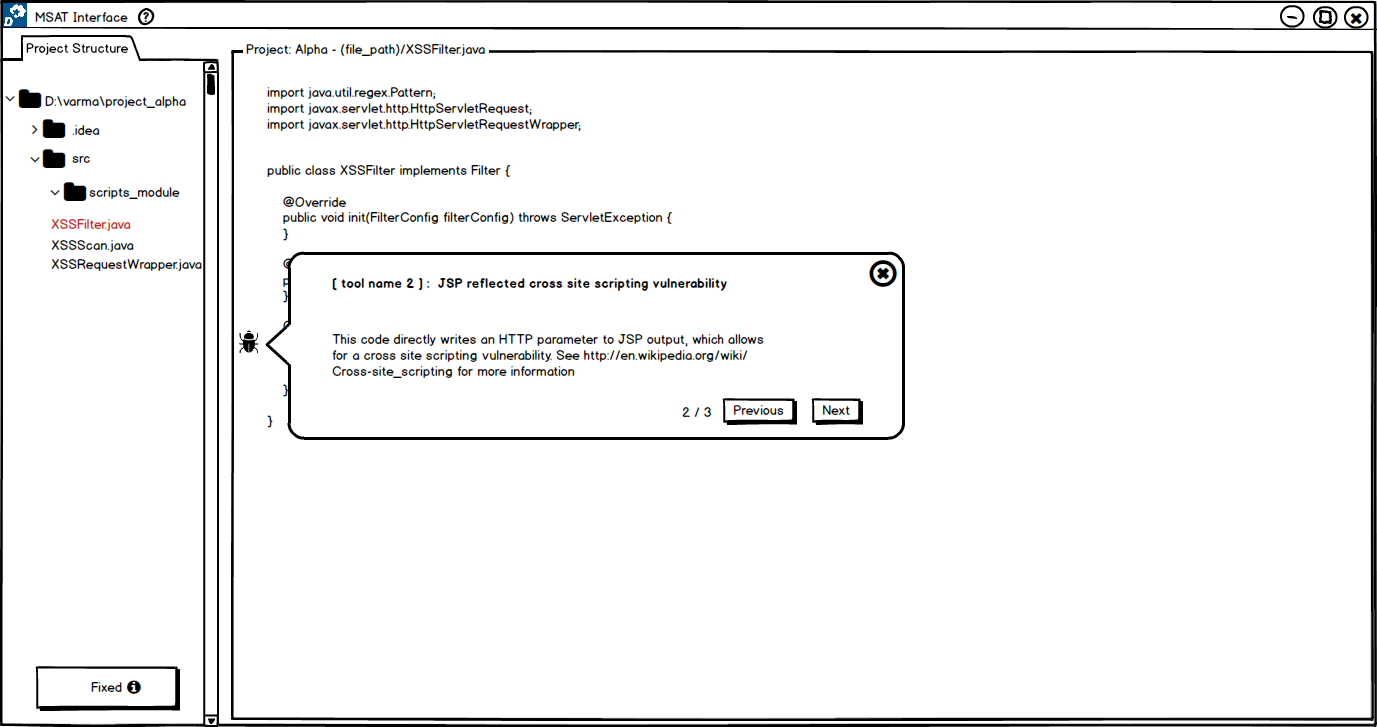
\includegraphics[width=\linewidth]{figures/solution_ideas_snaps/S31_next}
	\caption{An interface prototype showing ‘bug icon’ solution idea.}
	\label{fig:S31_next1}
\end{figure} 

The ‘list’ idea is about having a complete list of bugs in a file, and the user sees the list once he opens a file, then the bugs present in the file are shown in list. This idea could be well understood, looking at following \autoref{fig:S31_list1} or a complete prototype images added in appendix. \\


\begin{figure}[hbt!]
	\centering
	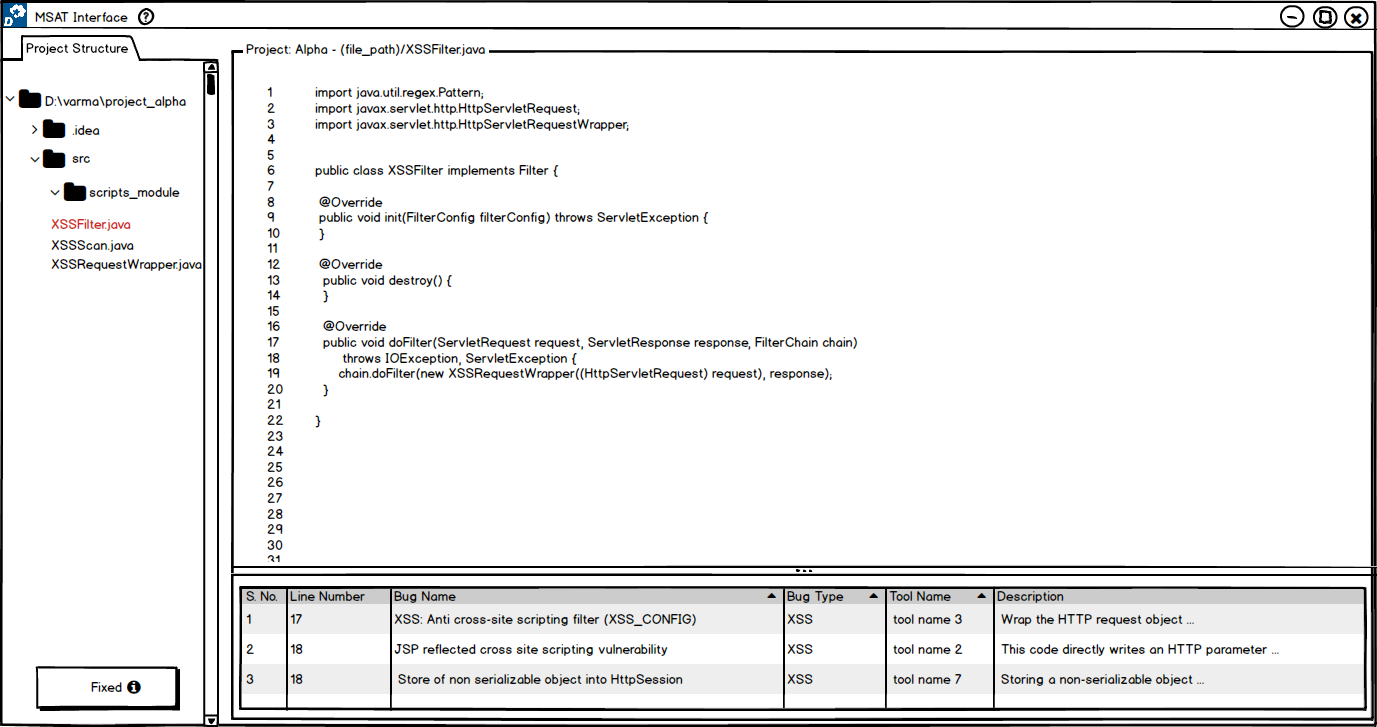
\includegraphics[width=\linewidth]{figures/solution_ideas_snaps/S31_list}
	\caption{An interface prototype showing ‘list’ solution idea.}
	\label{fig:S31_list1}
\end{figure} 

\clearpage

\textbf{Evaluation}: \\

Quantitative Results: \\

There are five user study participants. Every user has managed to perform the given task on the provided prototypes. With evaluation against the task success criteria, the result is 100 per cent. \\

Among the five users, two users chosen “bug icon” as a convenient solution idea for the given task and remaining three users has chosen “list” solution idea. The ratings of perceived usability of the bug icon solution idea in comparison to list solution idea by the five users are 8, 7, 9, 4 and 6. Similarly, the ratings of perceived usability of the list solution idea in comparison to bug icon solution idea by the five users are 7, 9, 7, 7 and 8. So, on an average, the perceived usability for bug icon solution idea is 6.8 rating and for list solution idea is 7.6 rating. \\

This numerical evaluation favours the list solution idea. \\

Qualitative Results: \\

Let us now investigate the reasoning behind the user’s choice of solution idea and respective ratings. The users who have chosen “bug icon” solution idea has mentioned that the design looks novel in their perspective. Further, it is better in seeing while working on a software tool, and they prefer limited things to see on a screen. Also, bug information provided on click gives better visualisation instead of looking for line number in list and then find the bug. One user was not able to know that clicking on the bug icon, and there would be a popup. Nevertheless, once known favoured the “bug icon” solution idea. \\

The users who have chosen “list” solution idea has mentioned that the provided user interface is predictable and more comfortable to locate. Further, it is much friendlier UI, can be looked at once instead of clicking multiple times in case of “bug icon”, in case of enormous codebase list benefits to see all bugs at one place whereas using bug icons needs scrolling up and down to see the results. \\

Users suggested a couple of ideas as an improvisation for “list” solution idea. One to have the code line highlighted by red colour along with list and the other is to display list on click of the icon, which focuses on multiple bugs in a line of code. \\

\begin{myboxi}{{\textbf{RQ 1-1: Do users prefer bug icons or list view for bugs in same file?}}}
	\\ \\ Users preferred list view as it is more comfortable and friendly UI. In case of huge codebase, bug icons solution idea would take more time in scrolling to identify bugs. \\
\end{myboxi}

\clearpage

\noindent \textbf{RQ 1-2: Do users prefer to see bugs one by one or at once in the context of multiple bugs at the same time?}: \\ \\

\textbf{Solution Ideas - Prototypes [ next, horizontal ]}: \\

The ‘next’ idea is about having a bug icon in the gutter, and user clicks to see the bug description at a particular line. Also, to see any other bugs in the same line, the user has to click on ‘next’ shown in bug description. This idea could be well understood, looking at following \autoref{fig:S31_next2} or a complete prototype images added in appendix. \\

The ‘horizontal’ idea is about showing a complete list of bugs that exist in a particular line of code as bug description boxes attached as top to bottom view, and the user sees it once he clicks on the bug icon in gutter. This idea could be well understood, looking at following \autoref{fig:S31_horizontal2} or a complete prototype images added in appendix. \\


\begin{figure}[hbt!]
	\centering
	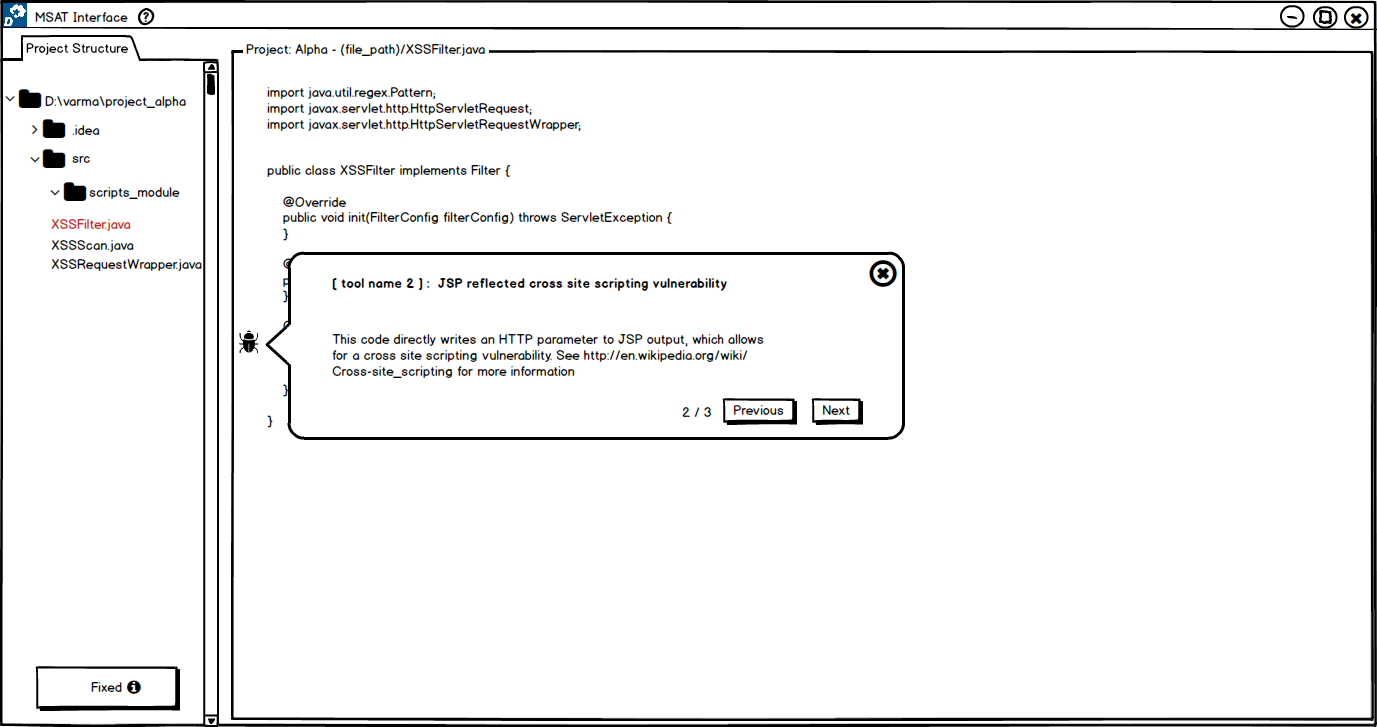
\includegraphics[width=\linewidth]{figures/solution_ideas_snaps/S31_next}
	\caption{An interface prototype showing ‘next’ solution idea.}
	\label{fig:S31_next2}
\end{figure} 

\begin{figure}[hbt!]
	\centering
	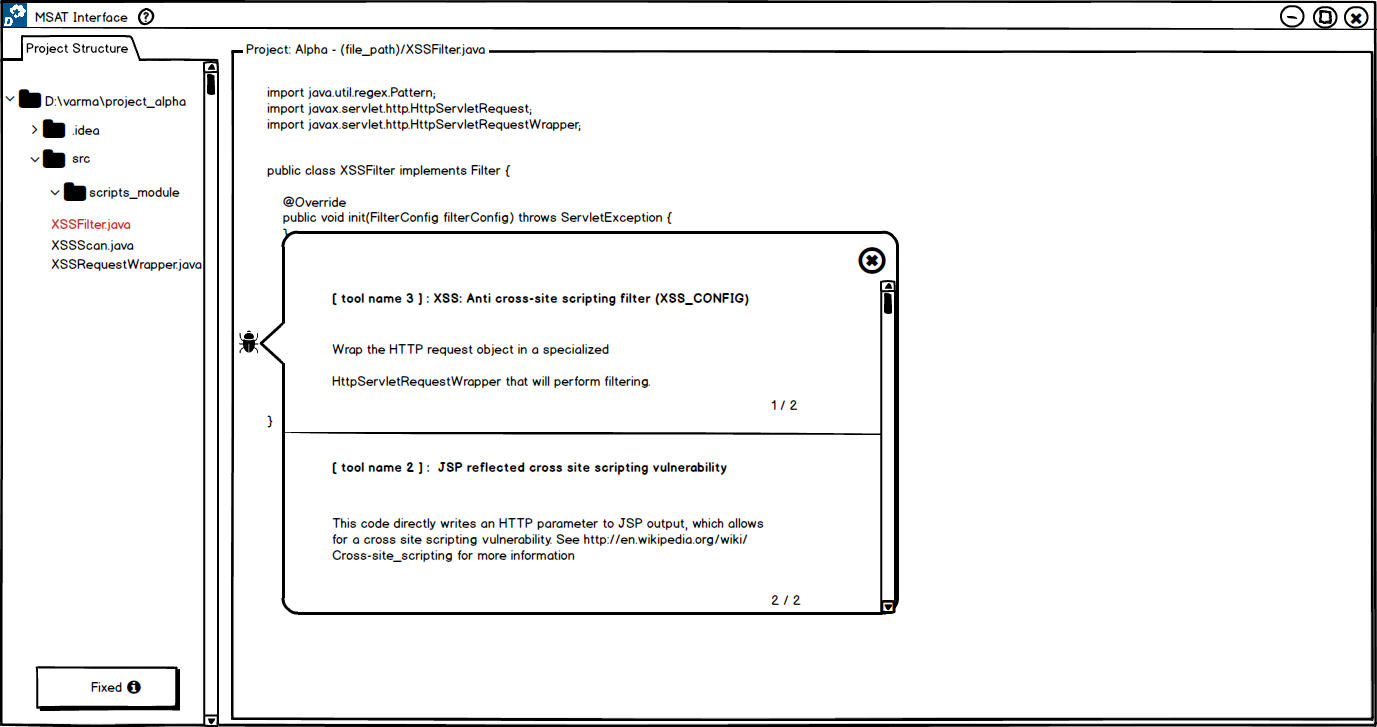
\includegraphics[width=\linewidth]{figures/solution_ideas_snaps/S31_horizontal}
	\caption{An interface prototype showing ‘horizontal’ solution idea.}
	\label{fig:S31_horizontal2}
\end{figure} 


\textbf{Evaluation}: \\

Quantitative Results: \\

There are five user study participants. Every user has managed to perform the given task on the provided prototypes. With evaluation against the task success criteria, the result is 100 per cent. \\

Among the five users, only one user-chosen “next” as convenient solution idea for given task and remaining four users has chosen “horizontal” solution idea. The ratings of perceived usability of the “next” solution idea in comparison to “horizontal” solution idea by the five users are 7, 8, 8, 4 and 7. Similarly, the ratings of perceived usability of the “horizontal” solution idea in comparison to “next” solution idea by the five users are 8, 9, 9, 6 and 6. So, on an average, the perceived usability for “next” solution idea is 6.8 rating and for “horizontal” solution idea is 7.6 rating. \\

This numerical evaluation favours the “horizontal” solution idea. \\

Qualitative Results: \\

Let us now investigate the reasoning behind the user’s choice of solution idea and respective ratings. The users who have chosen “next” solution idea has mentioned that it is preferred to see one bug at a time instead of looking at all bugs at once which might make the user miss some information. In case of going through each bug at a time will help the user to focus on more details such as quick tip/fix, references. \\

The users who have chosen “horizontal” solution idea has mentioned that having preference to see all bugs at once, scrolling down is much convenient. One other user-preferred “horizontal” solution idea specifically in case of multiple tools results for the sake of comparison instead of general preference where the user see one bug after other, understood and then move on to other. \\

One user suggested to have display of bugs in a separate window or in second screen instead of popping up on code view. The reasoning behind his suggestion is humans having tunnel vision focus which further helps to understand the code and correlate to bug finding. \\

\clearpage 

\begin{myboxi}{{\textbf{RQ 1-2: Do users prefer to see bugs one by one or at once in the context of multiple bugs at the same time?}}}
	\\ \\ Users preferred horizontal view as it helps in comparing results when using multiple tools. In general, users would like to go one by one and understand the results.
\end{myboxi}
\hfill \break

\noindent \textbf{RQ 1-3: Does vertical view help in getting an overview of the presence of multiple bugs over horizontal views?}: \\ \\

\textbf{Solution Ideas - Prototype [ horizontal, vertical ]}: \\

The ‘horizontal’ idea is about showing a complete list of bugs that exist in a particular line of code as bug description boxes attached as top to bottom view, and the user sees it once he clicks on the bug icon in gutter. This idea could be well understood, looking at following \autoref{fig:S31_horizontal3} or a complete prototype images added in appendix. \\

The ‘vertical’ idea is about showing a complete list of bugs that exist in a particular line of code as bug description boxes attached as left to right view, and the user sees it once he clicks on the bug icon in gutter. This idea could be well understood, looking at following \autoref{fig:S31_vertical3} or a complete prototype images added in appendix. \\ \\ \\ \\ \\


\begin{figure}[hbt!]
	\centering
	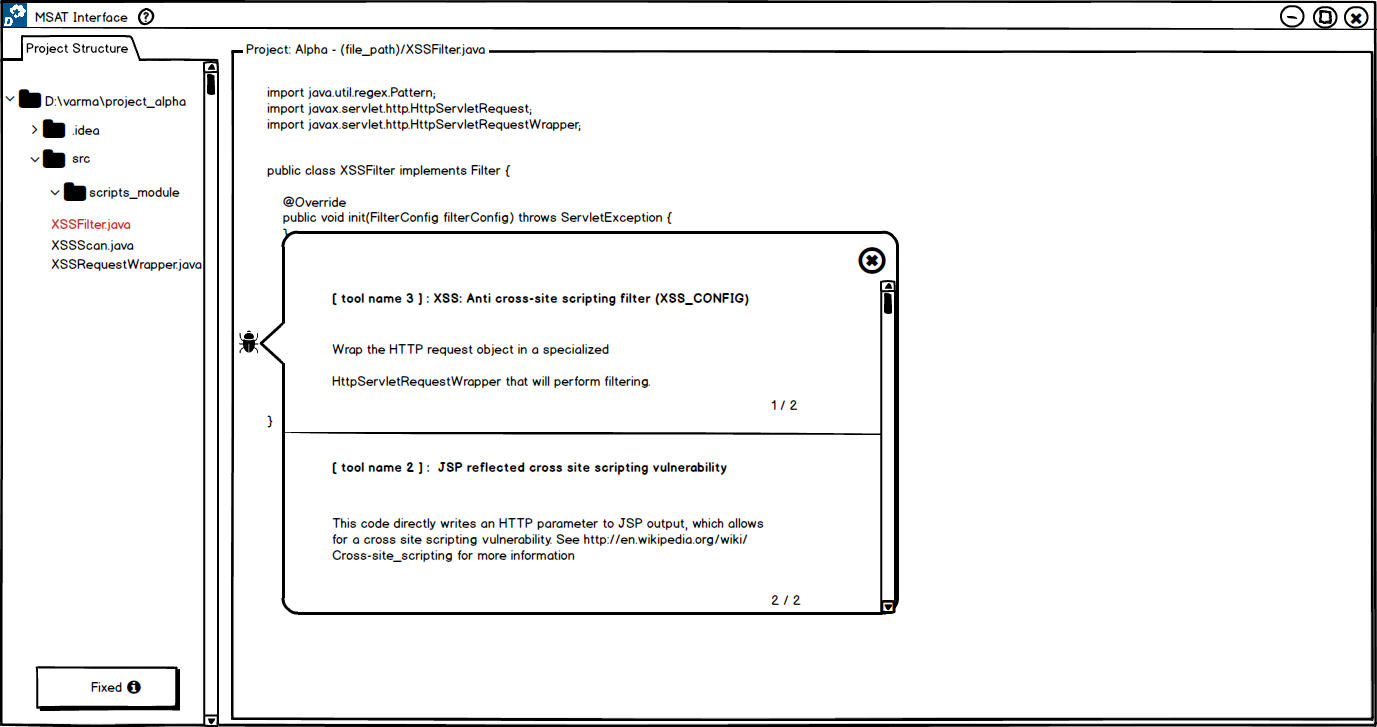
\includegraphics[width=\linewidth]{figures/solution_ideas_snaps/S31_horizontal}
	\caption{An interface prototype showing ‘horizontal’ solution idea.}
	\label{fig:S31_horizontal3}
\end{figure} 


\begin{figure}[hbt!]
	\centering
	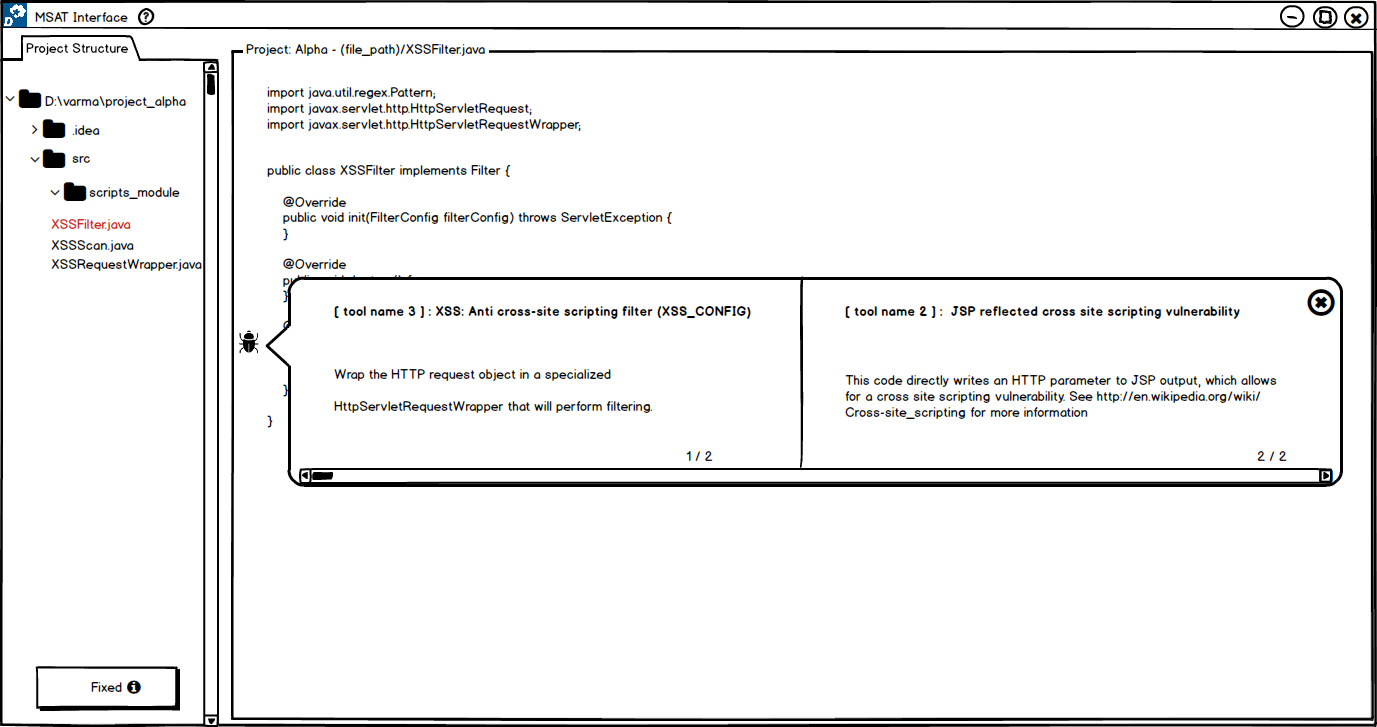
\includegraphics[width=\linewidth]{figures/solution_ideas_snaps/S31_vertical}
	\caption{An interface prototype showing ‘vertical’ solution idea.}
	\label{fig:S31_vertical3}
\end{figure} 


\textbf{Evaluation}: \\

Quantitative Results: \\

There are five user study participants. Every user has managed to perform the given task on the provided prototypes. With evaluation against the task success criteria, the result is 100 per cent. \\

Among the five users, three users chosen “horizontal” as convenient solution idea for given task and remaining two users has chosen “vertical” solution idea. The ratings of perceived usability of the “horizontal” solution idea in comparison to list solution idea by the five users are 9, 7, 9, 6 and 7. Similarly, the ratings of perceived usability of the “vertical” solution idea in comparison to “horizontal” solution idea by the five users are 8, 10, 7, 7 and 5. So, on an average, the perceived usability for “horizontal” solution idea is 7.6 rating and for “vertical” solution idea is 7.4 rating. \\

This numerical evaluation favours the “horizontal” solution idea. \\

Qualitative Results: \\

Let us now investigate the reasoning behind the user’s choice of solution idea and respective ratings. The users who have chosen “horizontal” solution idea has mentioned that the scrolling effect got used to, i.e., top to bottom scrolling in comparison to vertical which needs left to right scrolling, vertical display gives notion of hiding the code. \\ 
The users who have chosen “vertical” solution idea has mentioned that glancing from left to right is easy, just better to look in one line, best preferred on touch screen and landscape view display which makes easier to scroll. \\

In case of issue with covering of code by the popup views, users suggested to either have a separate view or to display popup box under the bug line and before the next code line. \\

\begin{myboxi}{{\textbf{RQ 1-3: Does vertical view help in getting an overview of the presence of multiple bugs over horizontal views?}}}
	\\ \\ The users mostly prefer horizontal view solution idea as they got used to such proposed UI concerning scrolling. In case of vertical view solution idea, users felt it is best suited for more landscape screens and touch screens.
\end{myboxi}
\hfill \break

\noindent \textbf{RQ 1-4: Do users prefer for table view over text description shown for multiple bugs at a line of code?}: \\ \\

\textbf{Solution Ideas - Prototype [ horizontal, table ]}: \\

The ‘horizontal’ idea is about showing a complete list of bugs that exist in a particular line of code as bug description boxes attached as top to bottom view, and the user sees it once he clicks on the bug icon in gutter. This idea could be well understood, looking at following \autoref{fig:S31_horizontal4} or a complete prototype images added in appendix. \\


\begin{figure}[hbt!]
	\centering
	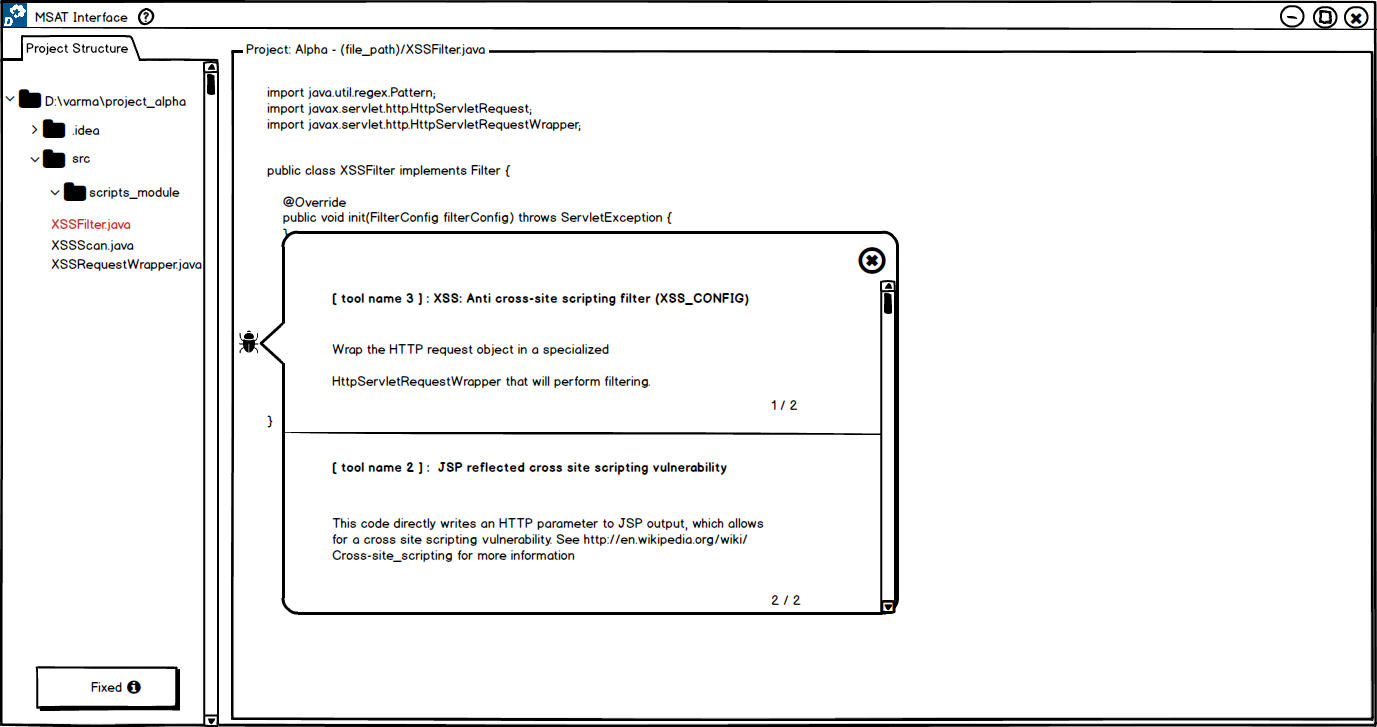
\includegraphics[width=\linewidth]{figures/solution_ideas_snaps/S31_horizontal}
	\caption{An interface prototype showing ‘horizontal’ solution idea.}
	\label{fig:S31_horizontal4}
\end{figure} 

The ‘table’ idea is about showing a complete list of bugs in table format that exist in a particular line of code, and the user sees it once he clicks on the bug icon in gutter. This idea could be well understood, looking at following \autoref{fig:S31_table4} or a complete prototype images added in appendix. \\

\begin{figure}[hbt!]
	\centering
	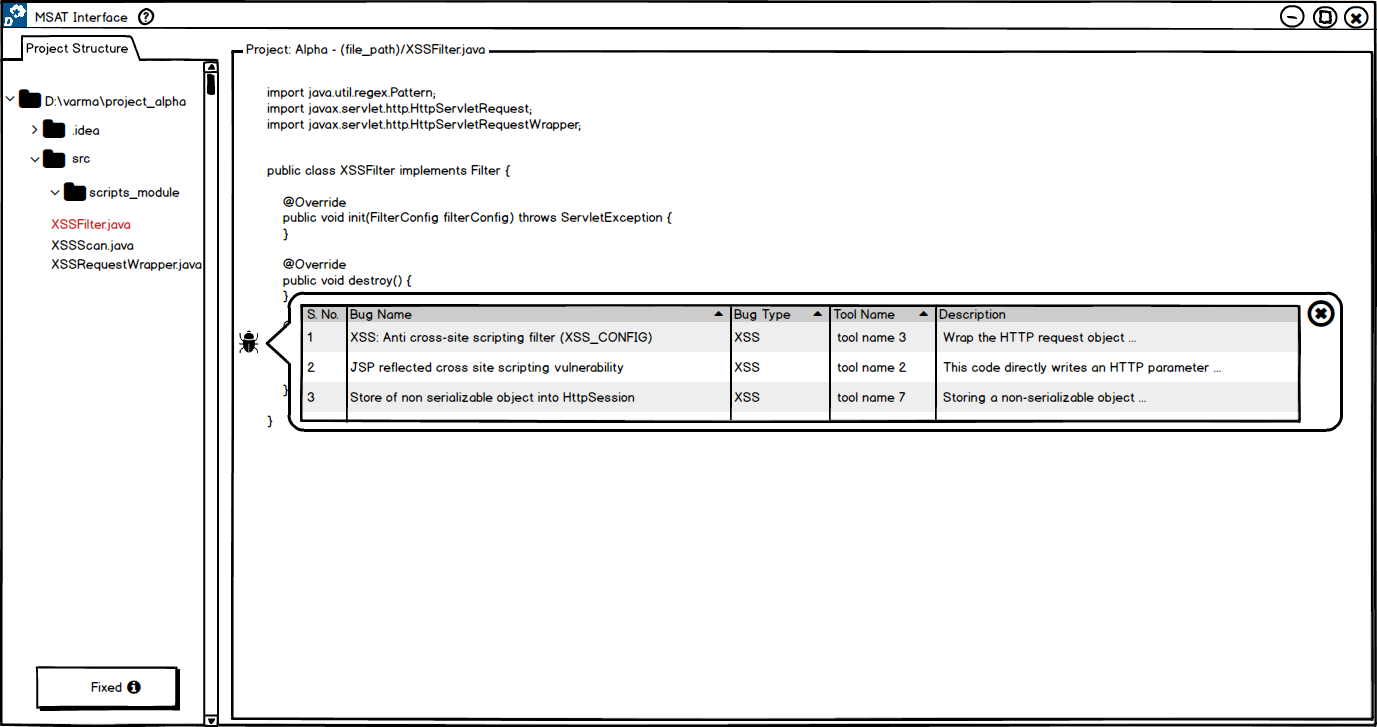
\includegraphics[width=\linewidth]{figures/solution_ideas_snaps/S31_table}
	\caption{An interface prototype showing ‘table’ solution idea.}
	\label{fig:S31_table4}
\end{figure} 


\textbf{Evaluation}: \\

Quantitative Results: \\

There are five user study participants. Every user has managed to perform the given task on the provided prototypes. With evaluation against the task success criteria, the result is 100 per cent. \\

Among the five users, all users chose “table” as convenient solution idea for given task instead of “horizontal” solution idea. The ratings of perceived usability of the “horizontal” solution idea in comparison to “table” solution idea by the five users are 8, 7, 8, 6 and 6. Similarly, the ratings of perceived usability of the “table” solution idea in comparison to “horizontal” solution idea by the five users are 9, 10, 9, 8 and 7. So, on an average, the perceived usability for “horizontal” solution idea is 7 rating and for “table” solution idea is 8.6 rating. \\

This numerical evaluation favours the “table” solution idea. \\

Qualitative Results: \\

Let us now investigate the reasoning behind the user’s choice of solution idea and respective ratings. Interestingly, all the users preferring the “table” solution idea has mentioned that it is easy to sort by bug types with a given table column, saves from distraction, understandability. Further, easy comparison for everything one below the other with columns having separate attributes, looks good, more manageable for user to stay in the context of workflow. In contrast, horizontal descriptions with scrolling takes more space, and it would rather be difficult for staying in the context of workflow, table view is more compact, easy to see bugs at a time. \\

Further, one user suggested to have short descriptions in table view to make it smaller, and on click of particular bug, we can have a complete description. One other user suggested to have the popups display with table view for a bug line when user types the next line to it. This functionality depends if tools are configured to analyse on the fly. \\

\begin{myboxi}{{\textbf{RQ 1-4: Do users prefer for table view over text description shown for multiple bugs at a line of code?}}}
	\\ \\ Users preferred table view over text descriptions as it helps to sort the results, and it also supports comparison.
\end{myboxi}
\hfill \break

\noindent \textbf{RQ 1-5: In context of same bug identified but with different line numbers, would have ‘similar bugs’ in bug description with on click pops up similar bug description boxes at the identified line or a list at the bottom help user in locating actual line where bug exist?}: \\


This sub research question will have a new user scenario, task and success criteria but similar follow-up questionnaire used for previous four sub research questions. The particular user study process pattern is changed, as described below. \\

\textbf{User Scenario}: \\

In the same scenario as so far, while looking at bug info at an individual code line, now the user would like to see similar bugs in the code file. It is to overcome issues with tools reporting wrong line numbers which reporting the same bug by other tool or just for information. \\



\textbf{Task}: \\

What are the similar bugs reported in file ‘XSSFilter.java’? \\

\textbf{Success Criteria}: \\

User reports the names of bugs, i.e., XSS\_Config and JSP, reflected vulnerability. \\


\textbf{Solution Ideas - Prototype [ similar boxes, similar list ]}: \\

The ‘similar boxes’ idea is about showing similar bugs as separate popups when user wants to find similar bugs in the same file by clicking on ‘similar’ named link in a bug description box. This idea could be well understood, looking at following \autoref{fig:S31_similar_boxes} or a complete prototype images added in appendix. \\

\begin{figure}[hbt!]
	\centering
	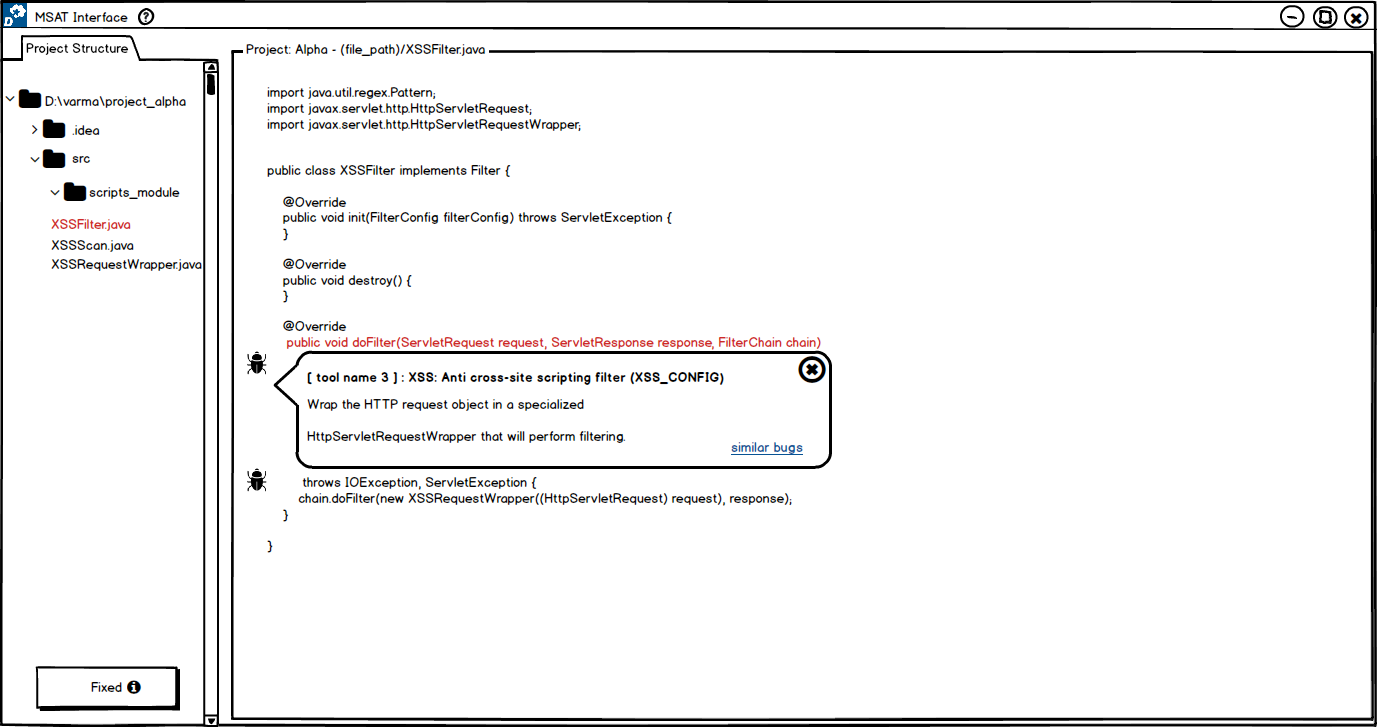
\includegraphics[width=\linewidth]{figures/solution_ideas_snaps/S31_similar_boxes}
	\caption{An interface prototype showing ‘similar boxes’ solution idea.}
	\label{fig:S31_similar_boxes}
\end{figure} 

The ‘similar list’ idea is about showing similar bugs as a list when user wants to find similar bugs in the same file by clicking on ‘similar’ named link in a bug description box. This idea could be well understood, looking at following \autoref{fig:S31_similar_list} or a complete prototype images added in appendix. \\ \\


\begin{figure}[hbt!]
	\centering
	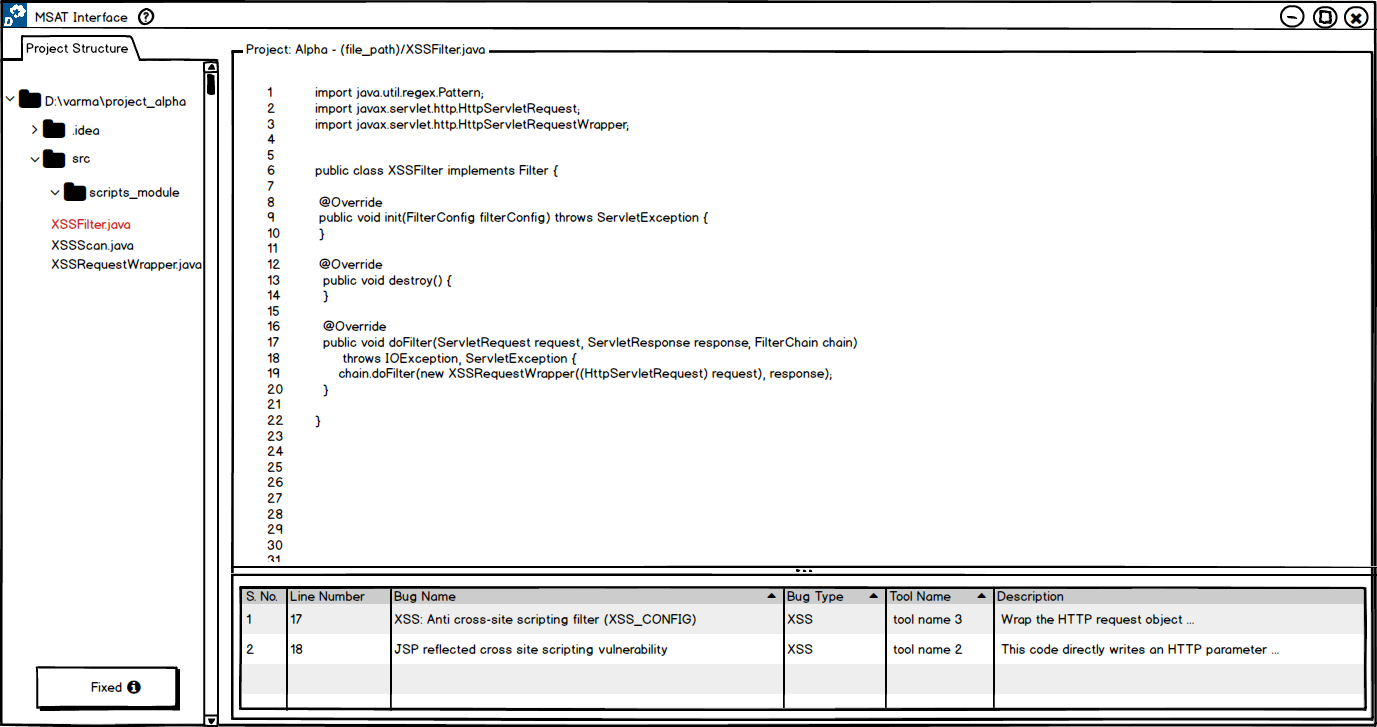
\includegraphics[width=\linewidth]{figures/solution_ideas_snaps/S31_similar_list}
	\caption{An interface prototype showing ‘similar list’ solution idea.}
	\label{fig:S31_similar_list}
\end{figure} 


\textbf{Evaluation}: \\

Quantitative Results: \\

There are five user study participants. Every user has managed to perform the given task on the provided prototypes. With evaluation against the task success criteria, the result is 100 per cent. \\

Among the five users, only one user-chosen “boxes” as convenient solution idea for given task and remaining four users has chosen “list” solution idea. The ratings of perceived usability of the “boxes” solution idea in comparison to “list” solution idea by the five users are 8, 7, 7, 5 and 5. Similarly, the ratings of perceived usability of the “list” solution idea in comparison to “boxes” solution idea by the five users are 7, 9, 8, 6 and 8. So, on an average, the perceived usability for “boxes” solution idea is 6.4 rating and for “list” solution idea is 7.6 rating. \\

This numerical evaluation favours the “list” solution idea. \\


Qualitative Results: \\

Let us now investigate the reasoning behind the user’s choice of solution idea and respective ratings. The users who have chosen “boxes” solution idea has mentioned that it is more accessible to correlate, easy to read by having more space for bug description. \\

The users who have chosen the “list” solution idea has mentioned that having two multiple icons on the same line is confusing to understand which one it is referring. Also, prefers list for simplicity, somewhat confusing when lines are moved down while display bug description popups in between code lines. Further,  better option in viewing similar bugs reported by all tools in a list on click in comparison to showing additional popup boxes as they are confusing, better to see everything at once as another option is time-consuming and a little bit confusing. \\

Further, one user suggested to have a respective code line highlighted in red colour or bug icon in addition to displaying similar bugs in a list. Other user says when the user fixes a bug reported by a tool, then interface should also not show the similar bugs reported by other tools. \\

\begin{myboxi}{{\textbf{RQ 1-5: In context of same bug identified but with different line numbers, would have ‘similar bugs’ in bug description with on click pops up similar bug description boxes at the identified line or a list at the bottom help user in locating actual line where bug exist?}}}
	\\ \\ Users preferred list solution idea as with additional popups; it would be confusing and time-consuming. \\
\end{myboxi}


Let us switch to the second main question.

\subsubsection{RQ 2: What feedback works to know that bug fixing is on-going?}

As part of this primary research question, we are going to evaluate the five feedback mechanisms proposed in previous user experience design cycle. These are animation, progress bar, pending status popup, status spinner and alert in our designed MSAT-UI ( Multiple Static Analysis Tools – User Interface ) in comparison to existing scenario where multiple tools have different user interfaces. In preparation, for this evaluation, a JavaScript software project is set up and hosted on GitHub. We configured this project with three static analysis tools having three different native user interfaces, i.e., CLI ( Command Line Interface ), IDE ( Integrated Development Environment ) and WEB interface. The analysis tools chosen for CLI, IDE and WEB based are ESLint, IntelliJ + SonarLint and SonarCloud respectively. \\

A demonstration of both scenarios is given to user wherein one scenario we presented a merged prototype with five feedback mechanisms and other scenario with a JavaScript project and walkthrough its respective analysis results. In order to help the user better understand the existing scenario and evaluate accurately against proposed MSAT-UI, similar to previous user study process pattern, a user scenario, couple of tasks with their success criteria and next with follow up questionnaire. \\

This approach helps to evaluate sub research questions, i.e., \\

\begin{enumerate}
\item How usable are each feedback functionality compared to the scenario of using unified UI to native UIs?
\item Does alert notification help in fixing more bugs in contrast to its absence in current tools UI?
\item Does MSAT UI with five different mechanisms helps in fixing the bugs in a faster way in comparison to using multiple tools with native user interfaces?
\item Does MSAT UI with five different mechanisms helps in fixing more bugs in comparison to using multiple tools with native user interfaces?
\end{enumerate}

\textbf{User Scenario}: \\

Assume the user as a software developer working on a project. The project is integrated with multiple tools independently with native user interfaces, i.e., CLI, IDE and WEB based. In contrast, the user have the project with a unified interface for them. \\


\textbf{Task 1}: \\

Identify the bugs in test.js file using CLI, IDE and WEB based analysis tools? \\

Success Criteria: \\

User reports the names of bugs shown from each interface. \\


\textbf{Task 2}: \\

Try to fix the bug of any unused-variable in index.js and see if the user fixes the bug or not? \\


Success Criteria: \\

User reports whether it got fixed or not. \\

\textbf{Follow up}: \\

Feedback features while working on a project integrated with multiple tools in the context of unified interface against native user interfaces. \\

Q. How do the user rate in terms of perceived usability ranging from O, be lower or absence of such feature to 10 be high for the respective feedback mechanism in comparison to existing scenario, i.e., having independent tools? \\
\begin{enumerate}
\item  How usable is animated icon feature? 
\item  How usable is progress bar feature? 
\item  How usable is status pending popup feature? 
\item  How usable is status spinner feature? 
\item  How usable is alert box feature? \\
\end{enumerate}

Further, we analyse the following three questions with the reasoning of their answer. \\

\begin{enumerate}
\item Do the user prefer alert box feedback when a bug fix is failed, which is absent in existing tools? Why?
\item Do these five feedback features with unified user interface help in fixing more bugs ( perceived usability )? Why?
\item Do these five feedback features with unified user interface help in fixing bugs faster ( perceived usability )? Why? \\
\end{enumerate}

\textbf{Evaluation}: \\

Quantitative results: \\

There are five user study participants. For task 1, only two users have managed to perform on the provided scenario. With evaluation against the task success criteria, the result is only 40 per cent. The reason behind why the other users have not able to do the task successfully is because two users were not able to remember the command to run analysis for CLI tool. Moreover, one user could not be able to navigate to individual project file in WEB interface. For task 2, all users managed to perform with complete 100 per cent result evaluated against the own task success criteria. \\

Let us now investigate each feedback mechanism and its respective rating. By first, with animation icons, the respective ratings in MSAT UI scenario is 8,10,7,10,7 with average rating 8.4 and whereas in Native-UI case is 0,0,0,0,0 with average rating 0. Next, with progress feedback, the respective ratings in MSAT UI scenario is 9,10,8,4,7 with average rating 7.6 and whereas in Native-UI case is 0,0,0,4,0 with average rating 0.8. Next, with pending status feedback, the respective ratings in MSAT UI scenario is 9,10,7,8,5 with average rating 7.8 and whereas in Native-UI case is 0,0,0,0,0 with average rating 0. Next, with status spinner feedback, the respective ratings in MSAT UI scenario is 9,10,8,9,8 with average rating 8.8 and whereas in Native-UI case is 0,10,0,10,0 with average rating 4. Finally, with alert feedback, the respective ratings in MSAT UI scenario is 9,10,9,9,9 with average rating 9.2 and whereas in Native-UI case is 0,0,0,0,0 with average rating 0. \\

So far, with numerical evaluation of perceived usability for each feedback mechanism proposed in the MSAT-UI outstands the existing scenario in terms of perceived usability. 
Further, all five users chose to have an alert box as a feedback mechanism feature. Next, all five users also agreed on having these five feedback mechanisms would help in fixing more bugs. However, only three users out of five agreed that these five feedback mechanisms would help in fixing more bugs. \\

Qualitative results: \\

Let us now investigate the reasoning behind the user’s preference and respective ratings. In case of choosing animated icons, i.e., icons are animated to indicate what the tool analyses, users felt they are useful if the system is slow in general. Also, it is easily identifiable on the screen, the plus point is to be aware of what analysis is running, and how many analysis is running, how many have completed. \\

In case of progress bar, users felt if analysis tools are too quick, then there is no need. Also, it is usable and useful thing to keep that. One user said if he starts the analysis manually, then it is useful or else useless as it could be diverting the attention if the user has panned for working on something else. One user expressed it has no use from his experience. Usually, he tends to wait until the progress gets complete, and he assumes progress bar, and such animations takes more resources than usual functionalities. In case of pending status feedback, users let it is helpful but not much necessary for end-user. In the case of status spinner, two users rated 10 for their usability in Native-UIs scenario as IDE usually has such feature. One user felt it is useful in knowing if analysis is running or not, whether started or not, only if run manually as then and only as in opposite case, he is not psychologically aware of it. \\

Now, in case of having alert feedback feature, users felt it is a good thing to have in the proposed one. It is used to have it to know that bug still exists and if so, try again to fix it. Also, it is preferred to have alert when tool decides the bug fix attempt is definite as to have psychological motivation which denotes positive feedback. On another side, some users felt it is annoying and so recommends to have slide popup somewhere corner instead of centre. It is more useful only when bug is very much important to get fixed as it indicates that it is not right if he move ahead without fixing it. It is irritating to have alert for small ones such as unused variables. \\
 
The reasonings of users for their choice, i.e., perceived usability of whether the proposed five feedback mechanisms help in fixing more bugs are such as, users will be more attentive. If user follow this practice, it would be more helpful; alert feedback helps in case of fixing more bugs whereas others show the status, other user says the same reasoning with alert saying when the tool decides the bug fix is negative. So he could work on it again. Further, status bar helps to know the time for analysing. Alert is helpful in the scenario of multiple software components by showing the existence of bugs in a microservice. Also, it is helpful in case of manual analysis. On the other side, one user felt as he generally checks before committing. So there is no much use case having these feedbacks.  \\

The reasonings of users for their choice, i.e., perceived usability of whether the proposed five feedback mechanisms help in fixing the bugs faster are such as, it helps by having direct visualisation of what is going on with these feedbacks. As an example, with progress bar user can wait and have patience, instead of working on something and making the system gets hanged. Also, ‘alert’ helps in this case where others show merely statistics. Status and progress bar helps to know the assumption time to complete analysis which anyhow depends on time taken by tool and not about fixing the bugs faster. It saves time in fixing the bugs as the user interface is essential for beginners in comparison to experts capable of working on a command-line interface. Interestingly, one user expressed his opinion that by only understanding what the bug is, it helps to fix a bug in a faster way. \\

\begin{myboxi}{{\textbf{RQ 2-1: How usable are each feedback functionality compared to the scenario of using unified UI to native UIs?}}}
	\\ \\ Each proposed feedback play an essential role in providing the information to the user. Some are absent in existing tools.
\end{myboxi}

\begin{myboxi}{{\textbf{RQ 2-2: Does alert notification help in fixing more bugs in contrast to its absence in current tools UI?}}}
	\\ \\ Users felt it as useful to have. As in case of success, it helps the developer have positive fulfilment in fixing the bug and in case of failure, the developer could re-try the bug fix again easily. \\
\end{myboxi}

\begin{myboxi}{{\textbf{RQ 2-3: Does MSAT UI with five different mechanisms helps in fixing the bugs in a faster way in comparison to using multiple tools with native user interfaces?}}}
	\\ \\ With the help of direct visualisations provided by the proposed feedbacks, users felt it is possible. Notably, ‘alert’ is helpful to try again to fix the bug immediately in case of bug fix fail. \\
\end{myboxi}

\begin{myboxi}{{\textbf{RQ 2-4: Does MSAT UI with five different mechanisms helps in fixing more bugs in comparison to using multiple tools with native user interfaces?}}}
	\\ \\ Users will be attentive with the provided feedbacks, and that assists in fixing more bugs. 
\end{myboxi}
\hfill \break

Let us switch to the final main question. \\

\subsubsection{RQ 3: How to carry traceability of bug fixing?}

As part of this primary research question, we evaluate the solution ideas of presenting the traceability scenario. In a user study, once we explain the concept of traceability to the user, and then present the following User Scenario, couple of Tasks which has their success criteria and finally, a follow-up questionnaire. \\

We evaluate the following sub research questions in this context. \\

\begin{enumerate}
\item Do users prefer having multiple windows to single window in tracing previous bug fixes in a method?
\item Do users be able to keep up in state of workflow as tools scale?
\item While tracing previous bug fixes in a method, do users prefer a table view to a before/after windows?
\end{enumerate}


\textbf{User Scenario}: \\

In the same scenario as so far, user notices there are some bugs fixed earlier in the same method. He/she would like to know what they are and so this might help in maintaining the method to be bug-free by not re-introducing old bugs again. \\

There are two solution ideas. One idea is to have a multiple window showing both before and after code changes of an analysis bug finding that happened in a section of code, i.e., in a method. This idea could be well understood, looking at following \autoref{fig:S33_multiple} or a complete prototype images added in appendix. \\


\begin{figure}[hbt!]
	\centering
	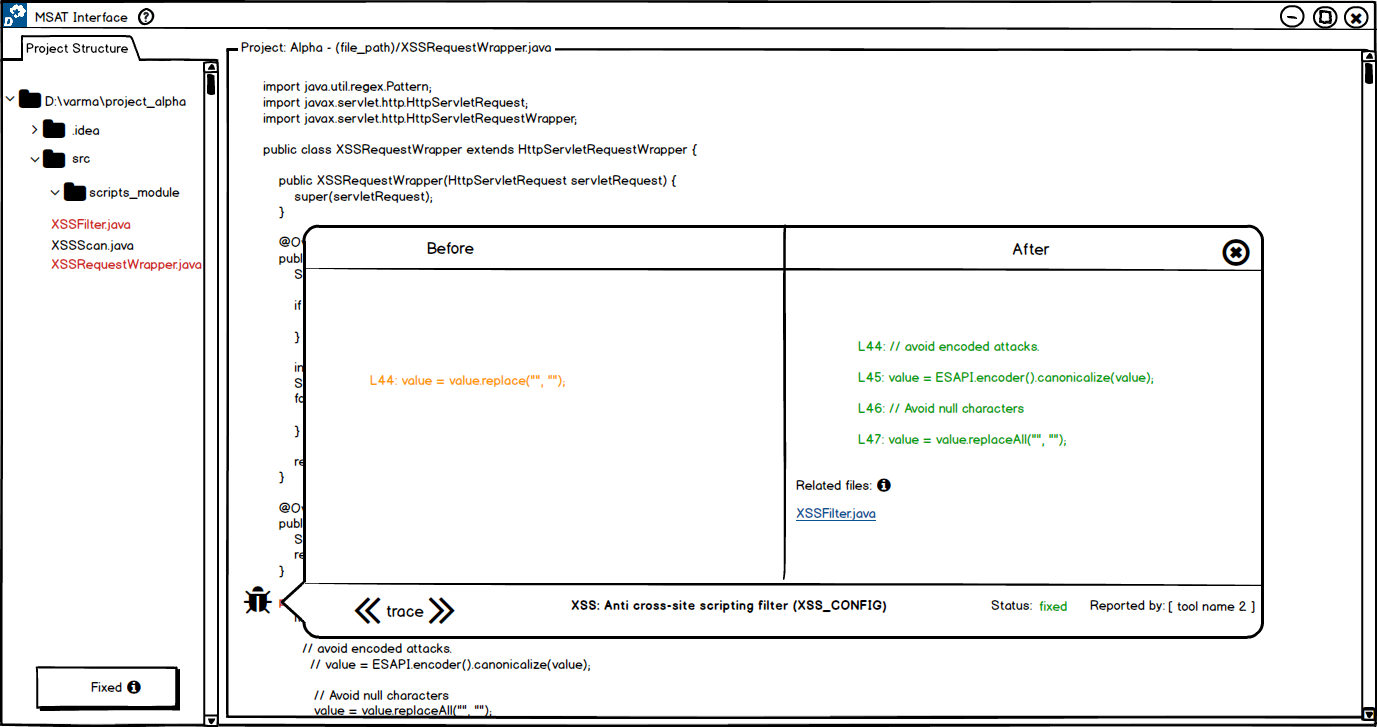
\includegraphics[width=\linewidth]{figures/solution_ideas_snaps/S33_multiple}
	\caption{An interface prototype showing ‘multiple window’.}
	\label{fig:S33_multiple}
\end{figure}

The other idea is to have a table view format of presenting the old bugs with the current one. This idea could be well understood, looking at following \autoref{fig:S33_table} or a complete prototype images added in appendix. We represent these two ideas to users as prototypes which are designed using Balsamiq. Next, the user is asked to perform the following two tasks on both prototypes. \\

\begin{figure}[hbt!]
	\centering
	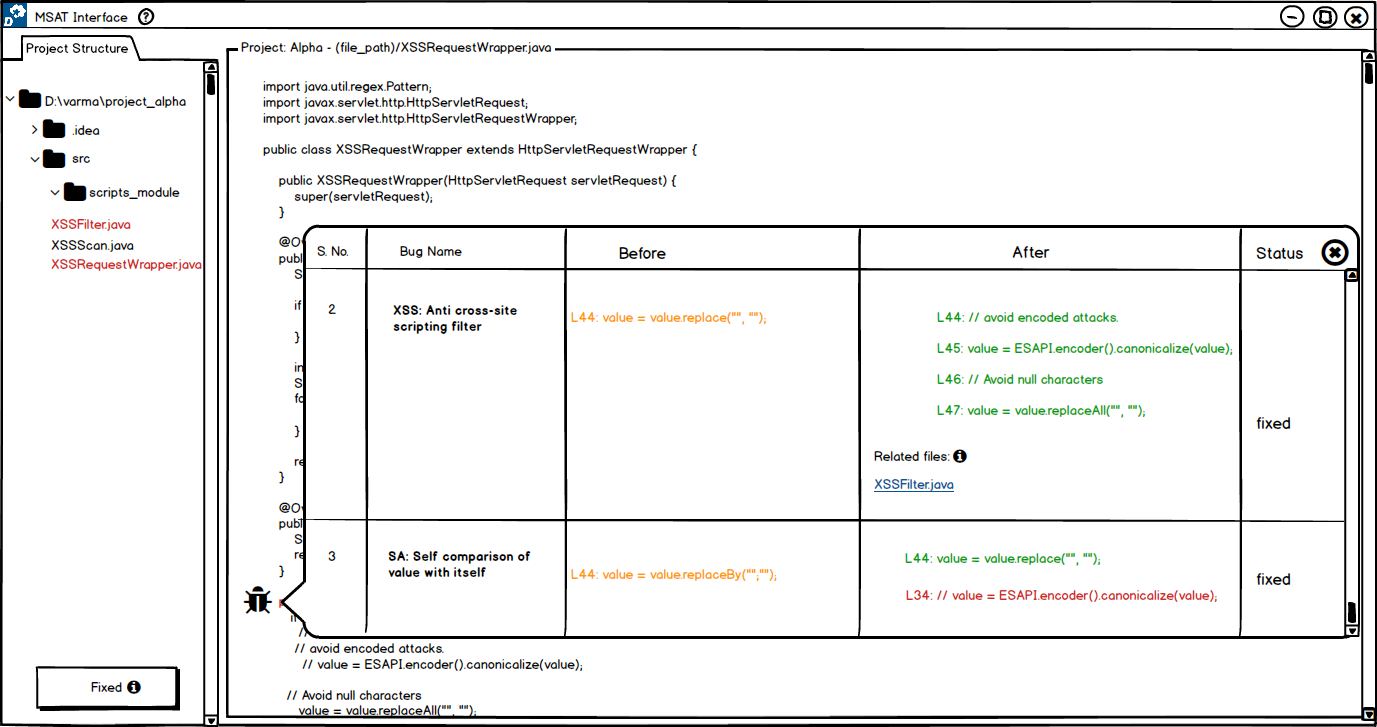
\includegraphics[width=\linewidth]{figures/solution_ideas_snaps/S33_table}
	\caption{An interface prototype showing ‘table view’.}
	\label{fig:S33_table}
\end{figure}

\textbf{Task 1}: \\ 

Identity how many bugs are fixed earlier in stripXSS method in file XSSRequestWrapper.java? \\ \\

Success Criteria: \\

User reports the number of bugs, i.e., 2. \\

\textbf{Task 2}: \\

What is the bug line reported as SA Bug-type earlier in stripXSS method in file XSSRequestWrapper.java? \\ \\

Success Criteria: \\
 
User reports the line as “L44: value = value.replaceBy("";"");”. \\

Once the user completed the tasks, we ask a set of following questionnaires in order to evaluate the solution ideas and the reasoning behind their choice of preference. \\

\textbf{Follow up}: \\

\begin{enumerate}
\item Among the two solution ideas presented, which one does the user feel convenient ( easy to use ) with for given tasks?
\item Why? What is the reason behind their choice?
\item How do the user rate in terms of perceived usability ranging from O, be lower or absence of such feature to 10 be high for both solution ideas in comparison to each other?
\item Which UI seems more scalable in this context of traceability helping the user in state of workflow?
\item Why? What is the reason behind their choice?
\end{enumerate}

\textbf{Evaluation}: \\

Quantitative results: \\

There are five user study participants. In case of first solution idea, i.e., multiple windows, for task 1, four users has managed to perform on the provided scenario. With evaluation against the task success criteria, the result of task success is 80 per cent, for task 2, three users has managed to perform on the provided scenario, and with evaluation against the task success criteria, the result of task success is 60 per cent. Next, in case of other solution idea, i.e., table list, for both task 1 and task 2, all users has managed to perform on the provided scenarios. With evaluation against the task success criteria, the result of task success is 100 per cent for both. \\

The perceived usability ratings provided by users for multiple windows solution ideas are 7, 9, 8, 10 and 8, with an average rating of 8.4. Similarly, for table list solution idea are 9,10,9,9 and 6, with an average rating of 8.6. Three users chose table list as their choice of convenience and remaining two users chose multiple windows.
As with the question of which interface solution idea is more scalable in comparison, four users chose table list, and one user chose the multiple windows idea. \\

Qualitative results: \\

Let us now examine the reason behind the user’s preference and their respective perceived usability ratings. As with task success, one user felt to have a precise declaration of colour coding used in solution ideas, i.e., for numbers (metrics) in table and different colours used for code lines. \\

The feedback for multiple windows solution idea by users is that they say it is simple, more evident when one type shown before/after rather than showing all at once as they are not related. Further, not confusing, users felt design to be novel for which one user got confused at the first impression but few seconds later understood the interface, colour coding needs clarification. One user said that although it requires documentation to understand initially with a learning curve, but still prefer it in comparison to table list. Interestingly, one other user mentioned that even the visualisation is good, but the user would still prefer alternative idea, i.e., table list. \\

Similarly, the feedback for table list solution idea by users are that it is convenient as the user can see everything in one screen and do not have to go and trace it back every time. Also, we can see or use solutions already applied then table is better to see parallelly than going front and back. Further, users do not need any help to understand the user interface, easy to use, easy to see at a time how the code is changed and what is the bug, maybe table view can take lot of page if more bugs and that needs scrolling which is not usable in perspective of one user. One user was not able to infer which line is buggy for task 2. \\

As an improvisation, also suggested by a couple of users that having colour is an add on, an excellent point to keep colours and so an info icon explaining the colour coding would suffice. One user stated he could be able to do similar tasks easily. One user suggested to have ‘bugs fixed earlier’ and ‘bugs need to be fixed’ as separate views to avoid confusion stated earlier as in precise with ‘before’ and ‘after’ columns used in multiple window solution idea design. \\

Next, in terms of scalability, the feedback on most users choice with table view is that it is more scalable to have at a glance. It is a better view than that of iterating through back and forth clicks, and we can see the bug details directly here, and even in case of more bugs, it is still better. One user suggests showing related bugs only to present one. Moreover, as it takes more time to browse through the multiple windows in case of more bugs, it would be better to add ‘go first’ and ‘go last’ kind of buttons to improve accessibility. \\

\begin{myboxi}{{\textbf{RQ 3-1: Do users prefer having multiple windows to single window in tracing previous bug fixes in a method?}}}
	\\ \\ Users preferred single window as it is easy to perceive results. \\
\end{myboxi}

\begin{myboxi}{{\textbf{RQ 3-2: Do users be able to keep up in state of workflow as tools scale?}}}
	\\ \\ Users can keep up in state of workflow as tools scale with the help of table view as it assists in having a glance in a single view. \\
\end{myboxi}

\begin{myboxi}{{\textbf{RQ 3-3: While tracing previous bug fixes in a method, do users prefer a table view to a before/after windows?}}}
	\\ \\ Users found both are useful, but in case of scalability, 4 out of 5 users preferred table view. \\
\end{myboxi}


\subsubsection{Post-test}

Before we end the user study, it would be interesting to know the importance and relevance of tool names in the context of using multiple tools for static analysis to a single project. \\

Questionnaire: \\
 
Q. Do the user prefer having tool names? \\

\textbf{Results}: \\

As with quantitative data, it is seen that out of 5 users, four users chose to have, and the remaining one user did not. Now, as with qualitative data, the feedbacks provided are that it does not affect much. However, if tool name is there, it is easy to remember which tool reported a particular bug and also helps to compare which tool performs better and so the user could discontinue the weak tool in future. One user stated that it helps in order to show the difference with which bug is identified by which tool, it also gives an idea about the effectiveness of findings based on tool specialised to cover. Other user in favour of having tool name stated that it is better to get as much information as possible being a developer or a tester. \\

One user says it could be optional as one tends to remember which tools he uses for a project, but in case of beginner, it could help. Alternatively, tool icons could suffice instead of tool names as users usually remember by objects. In the case of scenario, where tools could themselves have bugs as an example showing false positives, so later it can be investigated and report to tool developers. The user who is not in favour of having tool names said that it does not play any importance in solving the bug and does not even relate to efficiency of solving bugs more or in a faster way. \\ 


\begin{myboxi}{{\textbf{Do the user prefer having tool names?}}}
	\\ \\ It helps to determine the performance of tools. Also, users prefer to have more information when possible being a developer or tester. \\
\end{myboxi}

\section{Summary}

During the UX cycle 3, there are five users participated. The evaluation summarises answers for sub research questions as follows. For the first primary research question, display of results, to answer, do users prefer to see bugs one by one or at once in the context of multiple bugs at the same time,  users have chosen list as final solution idea than the bug icon solution idea. Although the bug icon idea is novel and helpful, but the list solution idea found to be more comfortable and friendlier UI. The other reason for choosing list is that it is ideal in scenario of large codebase in locating the bugs as other solution idea, i.e., bug icons needs more scrolling. Next to answer, do users prefer for table view over text description shown for multiple bugs at a line of code, users preferred the table view as it helps to compare the results in case of multiple tools. Although in general it is preferred for viewing one bug after other as it aids in understanding a bug and moving on to others. Next, to answer does vertical view help in getting an overview of the presence of multiple bugs over horizontal views, users preferred horizontal view as they got too used with the scrolling effect. Vertical views would be better in case of touch screen, and landscape view displays as it is easy to read from left to right. Next, to answer, do users prefer bug icons or list view for bugs in same file, all users favoured the table solution idea as with having list view as it is compact and easy to perceive the bug findings. Now In context of same bug identified but with different line numbers. To answer, would have ‘similar bugs’ in bug description with on click pops up similar bug description boxes at the identified line or a list at the bottom help user in locating actual line where bug exists. Users favoured the list solution idea as having additional popup boxes would be confusing and time-consuming. \\

For the second primary research question, feedback while bug fixing is on-going, the five proposed feedback mechanisms, i.e., animated icons, progress bar, pending status popup, alert and status are combined and evaluated against the real-time tools existed in market. The first sub research question about how usable are each feedback functionality compared to the scenario of using unified UI to native user interfaces. It is found out to be each feedback functionality that was proposed plays an essential role in its way of providing information to user. Some of the feedbacks are absent in real-time tools. Next to answer, does alert notification help in fixing more bugs in contrast to its absence in current tools UI, users felt it is good to have, although few felt it to be annoying. The alerts especially in success state help in giving positive encouragement to the user and in failure state, it helps the user to give one more try to fix the bug as he is also in same context. Now, let us see whether these five feedback mechanisms helps in fixing the bugs in a faster way. Users felt it be yes as they help in having direct visualisation of what is going on, and most users felt alert is more useful as it helps the user to try again to fix the bug immediately. Next, to answer, whether these five feedback mechanisms help in fixing more bugs, users felt so as they would be more attentive. \\

Finally, for the third primary research question, traceability of bug fixing, the first sub research question is about do users prefer having multiple windows to single window in tracing previous bug fixes in a method. Users expressed their opinions of choosing single window as it would be easy to perceive the results instead of going back and forth as shown with multiple windows solution idea.  Next, to answer, do users be able to keep up in state of workflow as tools scale, users mostly opted for table list as it aids in having a glance of everything in a single view. To the last sub research question, while tracing previous bug fixes in a method, do users prefer a table view to a before/after windows, users felt both are good ideas rated almost similar in usability. However, when it comes to scalability, 4 out of 5 users have chosen table list, although multiple windows visualisation is good. \\

Last but not the least, the question about whether the users prefer tool names or not. Out of five users, four users chose to have as it helps to remember which tool reported which bug and thereby analyse the tool performance and also it is needed by developer or tester to have as much information as possible. \\

\section{Lessons Learnt}

The primary limitations with this user study cycle are similar to previous UX cycle. We have taken care to the best extent possible. They are: \\

\begin{enumerate}
\item Mockup screens jump to next screen without of scope click, i.e., when the user clicked on keyboard input or with random mouse clicks, results in jumping of mockup screens. We expect that mockup screens navigate when the user clicks the desired link or button.
\item Animation effects are not possible with available prototype builder, i.e., Balsamiq.
\end{enumerate}

With this UX design cycle, we are able to cover maximum scenarios in using multiple tools and evaluate the promised solution ideas for each scenario. However, we still do have some exciting scenarios to look into, as mentioned in Chapter \ref{ch:futurework_report}, but as with time constraints, we open them for future work.

\emptypage